\documentclass[aspectratio = 169, 12pt]{beamer}

\input{preambles/preamble.tex}
\input{preambles/notation.tex}
\author{Jonathan Roth}
\title[Advanced DiD Mixtape Workshop]{Advanced DiD Mixtape Workshop \\ Introduction}

\begin{document}

\imageframe{figures/cover_intro.png}

\begin{frame}{Welcome!}
  \addtocounter{framenumber}{-1}

  Welcome to the Advanced Difference-in-Differences Mixtape Workshop!

  \medskip
  \begin{itemize}
    \item I am excited to learn with you all today.
  \end{itemize}

\end{frame}


\begin{frame}{Who Am I?}
  \begin{wideitemize}

    \item
    Assistant Professor of Economics at Brown University.

    \item
    I consider myself an \textit{applied econometrician}.

    \item
    The main goal of my research is to develop \textit{usable} tools that improve the quality of empirical work.

  \end{wideitemize}
\end{frame}


\begin{frame}{My DiD Journey}

  \begin{wideitemize}
    \item
    Early-on in graduate school, I was an aspiring labor economist running a lot of DiDs...

  \end{wideitemize}
  \centering
  \includegraphics[width =0.75\linewidth]{figures/act10-figure.png}

\end{frame}


\begin{frame}{My DiD Journey}
  \begin{wideitemize}
    \item
    I realized I had a lot of questions about the methodology of what I was doing.
    \begin{itemize}
      \item
            Should I believe parallel trends holds in this context?

      \item
            Why do I have pre-trends in some of my specifications but not others?

      \item
            Is it okay if I focus only on the specifications without pre-trends...?
    \end{itemize}

    \pause
    \item Pretty quickly I started writing methodological papers about these topics
    \begin{itemize}
      \item
            I never published the Act 10 paper -- oops!
    \end{itemize}

    \item But the goal of my research has always been to try to inform real-world analyses of economic topics

    \pause
    \item Today I hope to share with you some of the insights that I and others have learned over the last few years, with the \textbf{goal of helping you improve your research.}
    \begin{itemize}
      \item
            Focus on both theory and applying it in practice!
    \end{itemize}

  \end{wideitemize}
\end{frame}


\begin{frame}{(Approximate) Schedule for the day}
\begin{itemize}
	\item 10-11 Preliminaries \& The Canonical DiD Model
	\item 11-11:15 Break
	\item 11:15-12:30 Staggered treatment timing and heterogeneous treatment effects
	\item 12:30-1 Lunch
	\item 1-2 Coding Exercise
	\item 2-3:15 Violations of Parallel Trends
	\item 3:15-4:15 Coding Exercise
	\item 4:15-5:00 Open "Office Hour" for your DiD questions
\end{itemize}
\end{frame}


\begin{frame}{Course logistics}
  \begin{wideitemize}
    \item
    I strongly encourage you all to participate and ask questions!
    \begin{itemize}
      \item
            It's more fun for me and helps you learn better!
    \end{itemize}
    \item
    There are several ways that you can ask questions:

    \begin{wideitemize}
      \item
      Raise hand on Zoom

      \item
      Text question on Discord
    \end{wideitemize}

    \item
    I will pause periodically for you to ask live questions and to review messages on Discord
  \end{wideitemize}

\end{frame}


\begin{frame}{Introduction}
  \begin{wideitemize}
    \item
    \textbf{Difference-in-differences} (DiD) is one of the most popular strategies for estimating causal effects in non-experimental contexts.
    \medskip
    \begin{itemize}
      \item
            Used in over 20\% of NBER WPs \citep{currie_technology_2020}
    \end{itemize}

    \item
    The last few years have seen an explosion of econometrics on DiD, making it hard to keep up (sorry!)

    \item
    In Roth, Sant'Anna, Bilinski, and Poe (JOE, 2023), we attempted to synthesize the recent literature and provide concrete recommendations for practitioners


    \item
    This course is loosely based on the structure in that paper, focusing on staggered timing (Section 3) and violations of parallel trends (Section 4)
  \end{wideitemize}
\end{frame}


\begin{frame}{The simplest case}
	\begin{wideitemize}
		
		\item
		We will start a description of DiD in the simplest ``canonical'' case
		
		\item
		Why? Because recent DiD lit can be viewed as relaxing various components of the canonical model while preserving others
	\end{wideitemize}
	
	
	\pause
	In the canonical DiD model, we have:
	
	\medskip
	
	
	\begin{wideitemize}
		\item
		2 periods: treatment occurs (for some units) in period 2
		
		\item
		Identification of the ATT from parallel trends and no anticipation
		
		\item
		Estimation using sample analogs, equivalent to OLS with TWFE
		
		\item
		A large number of independent observations (or clusters)
	\end{wideitemize}
\end{frame}


\begin{frame}{Canonical DiD -- with math}
	\begin{wideitemize}
		\item
		Panel data on $Y_{it}$ for $t=1,2$ and $i = 1,...,N$
		
		\item
		\textbf{Treatment timing:} Some units ($D_i=1$) are treated in period $2$; everyone else is untreated $(D_i=0)$
		
		\pause
		\item
		\textbf{Potential outcomes:} Observe $Y_{it}(1) \equiv Y_{it}(0,1)$ for treated units; and $Y_{it}(0) \equiv Y_{it}(0,0)$ for comparison
	\end{wideitemize}
\end{frame}

\begin{frame}{Key Identifying Assumption - Parallel Trends}
	\begin{wideitemize}
		\item
		The \textbf{parallel trends} assumption states that if the treatment hadn't occurred, average outcomes for the treatment and control groups would have evolved in parallel
		$$\underbrace{ E[Y_{i2}(0) - Y_{i1}(0) \mid D_i =1] }_{\text{Counterfactual change for treated group}}= \underbrace{ E[Y_{i2}(0) - Y_{i1}(0) \mid D_i =0] }_{\text{Change for untreated group}} $$ 
		
		\pause
		\item
		The parallel trends assumption can also be viewed as a \textbf{selection bias stability} assumption:  
		$$\underbrace{ E[Y_{i2}(0)  \mid D_i =1] - E[Y_{i2}(0) \mid D_i=0] }_{\text{Selection bias in period 2}}= \underbrace{ E[Y_{i1}(0)  \mid D_i =1] - E[Y_{i1}(0) \mid D_i=0] }_{\text{Selection bias in period 1}} $$ 
		
		\item
		PT allows for there to be selection bias! But it must be stable over time
		
	\end{wideitemize}
\end{frame}

\begin{frame}{Visualizing PT}
	\begin{tikzpicture}[scale = 1.5]
		% Draw x-axis
		\draw[->] (0,0) -- (2.5,0) node[right] {Time};
		\draw (0,-0.1) -- (0,0.1);
		\draw (2,-0.1) -- (2,0.1);
		\node[below] at (0,-0.1) {1};
		\node[below] at (2,-0.1) {2};
		
		% Draw red dotted line
		\draw[red,dashed] (0,2) -- (2,2.5) node[above] {$E[Y(0) | Treated]$};
		
		% Draw blue solid line
		\draw[blue] (0,0.5) -- (2,1) node[midway,below=10pt] {$E[Y(0) | Control]$};
		
		% Add curly brace
		\draw[decorate,decoration={brace,amplitude=10pt}] (-0.2,0.5) -- (-0.2,2) node[midway,left=12pt] {Selection bias in period 0};
		
		% Add curly brace
		\draw[decorate,decoration={brace,amplitude=10pt,mirror}] (2.2,1) -- (2.2,2.5) node[midway,right=12pt] {Selection bias in period 1};
		
	\end{tikzpicture}
\end{frame}



\begin{frame}{Key identifying assumptions}
	\begin{wideitemize}
		\item
		\textbf{Parallel trends:}
		\begin{equation}
			\expe{ Y_{i2}(0) - Y_{i1}(0) \,|\, D_i = 1 } = \expe{ Y_{i2}(0) - Y_{i1}(0) \,|\, D_i = 0 } . \label{eqn: pt - 2 periods}
		\end{equation}
		
		
		\item
		\textbf{No anticipation:} $Y_{i1}(1) = Y_{i1}(0)$
		\begin{itemize}
			\item
			Intuitively, outcome in period 1 isn't affected by treatment status in period 2
			
			\item
			Often left implicit in notation, but important for interpreting DiD estimand as a causal effect in period 2
		\end{itemize}
	\end{wideitemize}
\end{frame}




\begin{frame}{Identification}
	\begin{wideitemize}
		\item
		\textbf{Target parameter:} Average treatment effect on the treated (ATT) in period 2
		
		$$\tau_{ATT} = E[Y_{i2}(1) - Y_{i2}(0) | D_i=1] $$
		
		\pause
		\item
		Under parallel trends and no anticipation, can show that
		
		$$\tau_{ATT} = \underbrace{(E[Y_{i2} | D_i = 1] - E[Y_{i1}| D_i =1])}_{\text{Change for treated}} - \underbrace{(E[Y_{i2} | D_i = 0] - E[Y_{i1}| D_i =0]) }_{\text{Change for control}},$$
		
		\noindent a ``difference-in-differences'' of population means
	\end{wideitemize}
\end{frame}

\begin{frame}{Visualizing Identification}
	
	\medskip	
	
	\begin{center}
		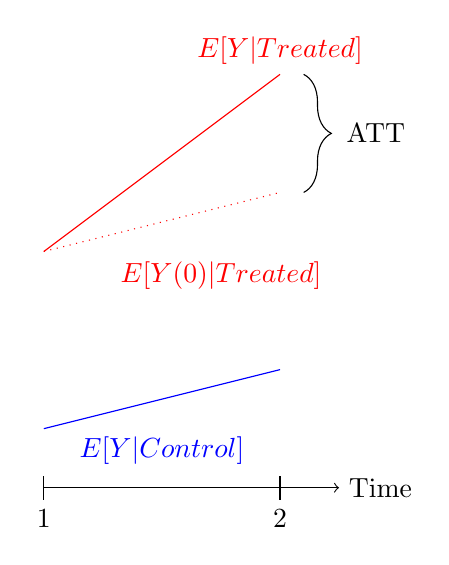
\begin{tikzpicture}[scale = 1.5]
			% Draw x-axis
			\draw[->] (0,0) -- (2.5,0) node[right] {Time};
			\draw (0,-0.1) -- (0,0.1);
			\draw (2,-0.1) -- (2,0.1);
			\node[below] at (0,-0.1) {1};
			\node[below] at (2,-0.1) {2};
			
			% Draw red dotted line
			\draw[red,dotted] (0,2) -- (2,2.5);
			
			\node[below,red] at (1.5,2) {$E[Y(0) | Treated]$};
			
			% Draw red dotted line
			\draw[red] (0,2) -- (2,3.5) node[above] {$E[Y | Treated]$};
			
			% Draw blue solid line
			\draw[blue] (0,0.5) -- (2,1) node[midway,below=10pt] {$E[Y | Control]$};
			
			% Add curly brace
			\draw[decorate,decoration={brace,amplitude=10pt,mirror}] (2.2,2.5) -- (2.2,3.5) node[midway,right=12pt] {ATT};			
		\end{tikzpicture}			
	\end{center}%
	
	
	
\end{frame}


\begin{frame}{Proof of Identification Argument}
	\begin{itemize}
		\item
		Start with
		\vspace{-3mm}
		$$E[Y_{i2}- Y_{i1}| D_i =1] - E[Y_{i2} - Y_{i1}| D_i =0]$$
		
		\pause
		\vspace{-3mm}
		\item
		Apply definition of POs to obtain:
		\vspace{-3mm}
		$$E[Y_{i2}(1) - Y_{i1}(1)| D_i =1] - E[Y_{i2}(0) - Y_{i1}(0)| D_i =0]$$
		
		\pause
		\vspace{-3mm}
		\item
		Use No Anticipation to substitute $Y_{i1}(0)$ for $Y_{i1}(1)$:
		\vspace{-3mm}
		$$E[Y_{i2}(1) - Y_{i1}(0)| D_i =1] - E[Y_{i2}(0) - Y_{i1}(0)| D_i =0]$$
		
		\pause
		\vspace{-3mm}
		\item
		Add and subtract $E[ Y_{i2}(0) | D_i =1] $ to obtain:
		\vspace{-3mm}
		\begin{align*}
			& \electricViolet{E[ Y_{i2}(1) - Y_{i2}(0) | D_i =1]} + \\
			& \hspace{1cm} \sun{\left[ (E[Y_{i2}(0) | D_i = 1] - E[Y_{i1}(0)| D_i =1]) - (E[Y_{i2}(0) | D_i = 0] - E[Y_{i1}(0)| D_i =0]) \right]}
		\end{align*}
		
		\pause
		\vspace{-3mm}
		\item
		Cancel the \sun{last terms} using PT to get $\electricViolet{E[Y_{i2}(1) - Y_{i2}(0) | D_i = 1] = \tau_{ATT}}$
	\end{itemize}
	
\end{frame}





\begin{frame}{Estimation and Inference}
	\begin{wideitemize}
		\item
		The most conceptually simple estimator replaces population means with sample analogs:
		$$\hat{\tau}_{DiD} = (\bar{Y}_{12} - \bar{Y}_{11}) - (\bar{Y}_{02} - \bar{Y}_{01}) $$
		\noindent where $\bar{Y}_{dt}$ is sample mean for group $d$ in period $t$
		
		\pause
		\item
		Conveniently, $\hat\tau_{DID}$ is algebraically equal to OLS coefficient $\hat\beta$ from
		\begin{equation}
			Y_{it} = \alpha_i + \phi_t + D_{it} \beta  + \epsilon_{it}, \label{eqn: TWFE-2-periods}
		\end{equation}
		\noindent where $D_{it} = D_i * 1[t=2]$. Also equivalent to $\beta$ from $\Delta Y_{i} = \alpha +  \Delta D_i \beta + u_{it}$.
		\pause
		\item
		\textbf{Inference:} And clustered standard errors are valid as number of clusters grows large
	\end{wideitemize}
\end{frame}

\begin{frame}{Characterizing the recent literature}
	We can group the recent innovations in DiD lit by which elements of the canonical model they relax:
	\medskip
	
	\begin{wideitemize}
		\item
		\textbf{Multiple periods and staggered treatment timing}
		
		\item
		\textbf{Relaxing or allowing PT to be violated}
		
		\item
		\textbf{Inference with a small number of clusters}
		
	\end{wideitemize}
	\medskip
	Will focus today on the first two
\end{frame}

\nocite{roth_whats_2023}

\backupbegin
\begin{frame}[allowframebreaks,noframenumbering,plain]{References}
  \bibliography{Bibliography.bib}
\end{frame}
\backupend
\end{document}
